% !TEX root = ../Masters.tex
\chapter{Distribution-based Grammar Evolution of L-systems}

% NEED TO DESCRIBE LIMITS TO NUMBER OF INSTRUCTIONS.

\section{Overview}
\label{sec:overview}
To generate L-system plants that are aesthetically pleasing, varied and could be used to create offspring similar to its parents (\textbf{RQ0}), an algorithm called Distribution-based Grammar Evolution of L-systems (DGEL) was developed.

The DGEL name consists of two parts that are essential to solve the three sub research questions: \textit{Grammar Evolution (GE)} and \textit{Distribution-based}.
It uses GE to evolve L-system plants because it allows the algorithm to use well-researched techniques for modifying or combining genes into new L-systems (\textbf{RQ1}).
As part of the GE process, there is a fitness function that evaluates how aesthetically pleasing a plant is, thus pushing the evolution towards aesthetically pleasing plants (\textbf{RQ2}).
It is distribution-based, meaning that different probability distributions for the L-system grammar can be used to generated varied plants (\textbf{RQ3}).

\begin{figure}
    \centering
    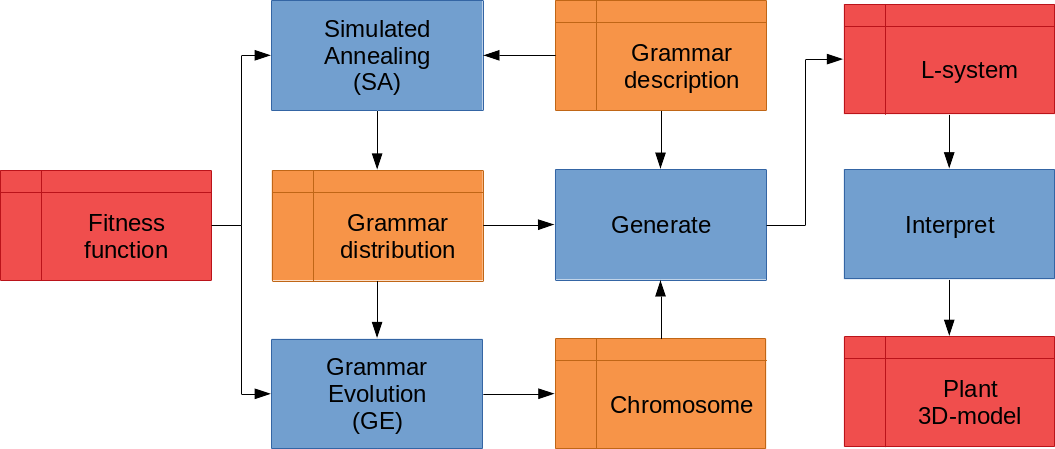
\includegraphics[width=1.0\textwidth]{figures/dgel}
    \caption[DGEL components and flow]{DGEL components and flow. Blue boxes represent processes and red boxes represent models. Grey boxes are logical collections of the components.}
    \label{fig:dgel}
\end{figure}

Figure~\ref{fig:dgel} illustrates the modules, processes and models of the DGEL algorithm.
It consists of two modules: \textit{Evaluation} and \textit{Generation}.
Evaluation evaluates how good an L-system plant is, and the Generation uses this information to generate good L-system plants.
The end result is a plant 3D model that is interpreted from an L-system.
The L-system is generated by a chromosome using a grammar distribution for a grammar description.
These three models: the grammar description, grammar distribution and the chromosome, together define the L-system.
All L-systems generated using the same grammar description, grammar distribution and chromosome will result in the exact same L-system, which also will be interpreted into the exact same plant 3D model.
GE is used to generate a good chromosome based on the grammar description, grammar distribution and a fitness function.
The grammar distribution is generated by Simulated Annealing (SA) based on the grammar description and a fitness function.
The fitness function models how aesthetically pleasing a plant is by assigning it score in range $[0, 1]$, where 0 is the worst, and 1 is the best.

\section{Representing an L-system with Grammar}
\label{sec:grammar}
As described, the L-systems in DGEL are represented by a chromosome, a grammar description and a grammar distribution.
If we assume a uniform grammar distribution, only a chromosome and a grammar description is required.

The grammar description, represented in a format such as the Backus Naur Form (BNF), describes the syntax of the L-system.
For example, it may describe that an L-system consists of a number of rules, each with a predecessor and successor, where a predecessor contains one character, etc.
The chromosome describes the choices to be made in the grammar description, for example how many rules there are, or which character the predecessor contains.
These choices are what creates the variations in the L-systems.
If there were no choices, there would only exist one single L-system.

This method of representing the L-systems was based on Beaumont and Stepney's work on applying GE to plant L-systems~\cite{2009Beaumont}, in addition to Ortega et al.'s work on applying it to fractal L-systems~\cite{2003Ortega}, and Ryan et al.'s introduction of GE~\cite{1998Ryan}.

While Ortega et al.\ and Beaumont and Stepney make assumptions about the grammar to significantly simplify it and reduce the search space~\cite{2003Ortega, 2009Beaumont}, the DGEL method uses a grammar that covers the largest search space reasonably possible.
To make the search space reasonable, there still have to be some limits.
The number of productions, string length, and number of characters for a variable were limited to a maximum of 20.
A higher number did not seem reasonable as no L-systems in the literature reviewed used larger numbers, and the search times for higher numbers started to become unreasonable long.

Additionally, to limit the complexity of L-systems, complex features such as leaves, flowers, branch segment width and more were not included.
Thus the grammar used can only produce the branches of a plant.
This is the most essential part of a plant, which can be expanded later by modifying only the grammar description.
Listing~\ref{lst:grammar} shows the actual grammar description used during the development and testing of the algorithm, while Listing~\ref{lst:grammar2} shows a grammar description that supports leaves and varying branch segment width.

\begin{lstlisting}[caption=ABNF grammar description used in DGEL, label=lst:grammar, float]
lsystem = axiom productions
axiom = string
productions = 1*20production
production = predecessor successor
predecessor = variable
successor = string
string = 1*20(symbol / stack)
stack = "[" string "]"
symbol = variable / operation
variable = %x41-55
operation = "+" / "-" / "^" / "&" / ">" / "<"
\end{lstlisting}

\begin{lstlisting}[caption=ABNF grammar description supporting leaves and varying branch segment width, label=lst:grammar2, float]
lsystem = axiom productions
axiom = string
productions = 1*20production
production = predecessor successor
predecessor = variable
successor = string
string = 1*20(symbol / stack / leaf)
symbol = variable / operation
variable = %x41-55
operation = "+" / "-" / "^" / "&" / ">" / "<" / "!"
stack = "[" string "]"
leaf = "['{+f-f-f+|+f-f}]"
\end{lstlisting}

To be able to use different grammar distributions, the chromosome representation is a different from that of Ryan et al.\ where each gene is an unsigned 8-bit integer and the choice to be made is the alternative index by the gene modulo the number of alternatives~\cite{1998Ryan}.
Each gene is still represented by an unsigned integer, but it is 32-bit instead of 8-bit, and the interpretation of the integer is different.

A gene in the DGEL chromosome can be viewed as an index into the value range of the 32-bit integer.
This value range, from $0$ to $2^{32}$, can be viewed as a line with segments representing each alternative in a rule in the grammar.
In the case of a uniform distribution the segments would be equal in length, while for a different distribution the lengths will differ.
The value of each gene in the chromosome is randomly picked from a uniform distribution, thus making the actual distribution dependent on the grammar distribution.

Figure~\ref{fig:gene} illustrates an example of this process.
A choice is to be made between $C$, $D$, $E$ and $F$ in the rule $A \rightarrow C / D / E / F$.
A chromosome of length 4 containing 4, 3, 0 and 7 is used, and the next gene to be used in the chromosome is the second position, i.e.\ the value 3.
Each gene is a 3-bit unsigned integer, thus having 8 possible values in range $[0, 8)$.
Since there are four alternatives, and a uniform distribution is used, the 3-bit value range is split into four segments of 2 values.
The gene value 3 maps into the second segment, which maps to the second alternative in the rule, i.e.\ $D$.
This process would then continue with the next gene, 0, on the $D$ rule.

\begin{figure}
    \centering
    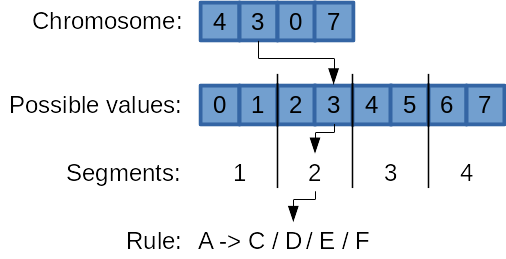
\includegraphics[width=0.8\textwidth]{figures/gene}
    \caption[Example grammar alternative selection from gene]{Example grammar alternative selection from gene. In the figure, the gene is a 3-bit integer, and thus has 8 possible values.}
    \label{fig:gene}
\end{figure}

\section{Interpreting L-systems Into Plant 3D Models}
As seen in Figure~\ref{fig:dgel}, after an L-system has been generated, it needs to be interpreted into a 3D-model such that people may see the plant.
Turtle interpretation is used to do this~\cite{2012Prusinkiewicz}, as it is a popular method used in the literature.
A 3D version of the turtle interpretation is used, where the turtle can draw lines with \textit{F}, and rotate around three axes using \textit{-} and \textit{+} for yaw, \textit{\textasciicircum} and \textit{\&} for pitch, and \textit{<} and \textit{>} for roll.
The bracket operators, \textit{[} and \textit{]}, are used to create branch bases.
Table~\ref{tab:turtle-cmd} shows a complete overview of the characters and their operations, including extra operators used for more control and features like leaves (e.g.\ Listing~\ref{lst:grammar2}).

\begin{table}
    \centering
    \begin{tabular}{| c | l |}
    \hline
    \textbf{Character} & \textbf{Operation} \\ \hline
    F & Draw line forward \\ \hline
    + & Yaw left \\ \hline
    - & Yaw right \\ \hline
    \textasciicircum & Pitch up \\ \hline
    \& & Pitch down \\ \hline
    < & Roll left \\ \hline
    > & Roll right \\ \hline
    | & Yaw 180° \\ \hline
    [ & Push state \\ \hline
    ] & Pop state \\ \hline
    \{ & Begin surface \\ \hline
    \} & End surface \\ \hline
    ! & Decrease width \\ \hline
    ` & Next color \\ \hline
    f & Draw line forward \\
    \hline
    \end{tabular}
    \caption[Turtle interpretation of L-system characters]{Turtle interpretation of L-system characters. \textit{f} does the same as \textit{F}, but is not allowed as a predecessor int the grammar such that it can not recurse.}
    \label{tab:turtle-cmd}
\end{table}

The actual 3D model created from this interpretation is kept as simple as possible while still trying to look somewhat natural.
The branch segments (created by the \textit{F} character) are brown stretched cubes.
Leaves are green flat surfaces.
An example can bee seen in Figure~\ref{fig:example-model}.

\begin{figure}
    \centering
    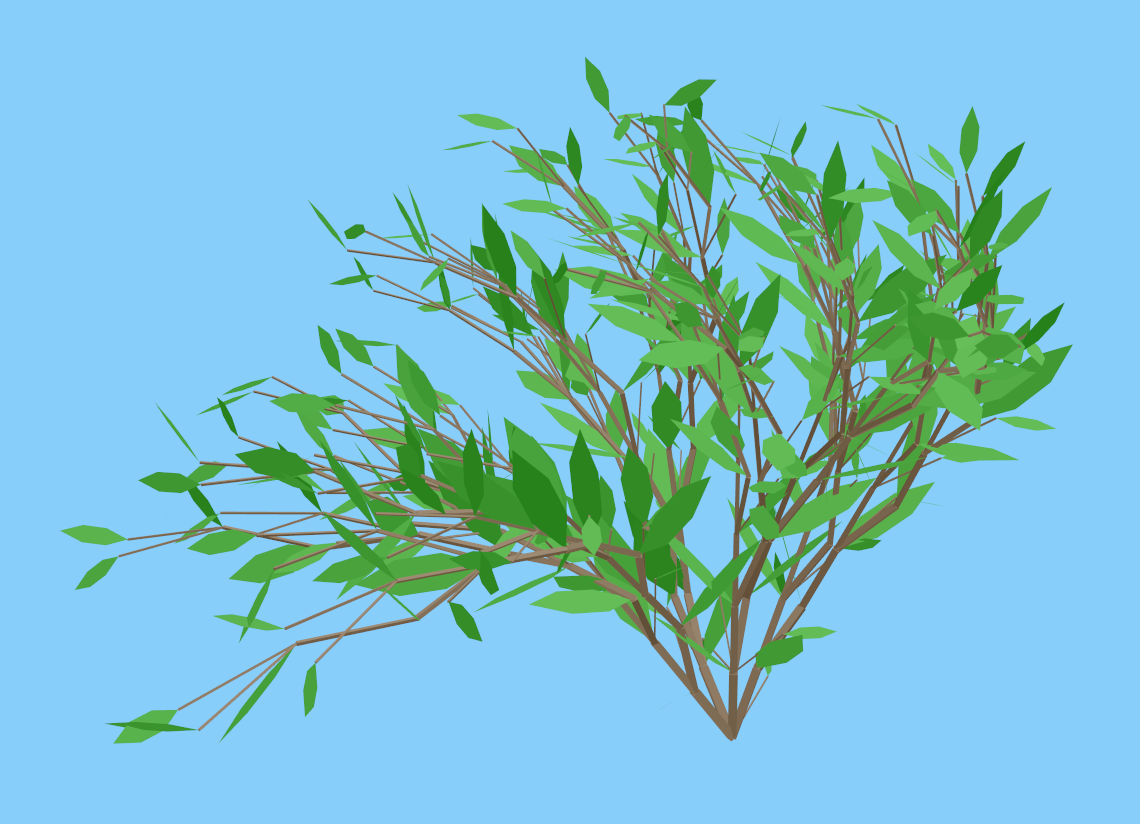
\includegraphics[width=1.0\textwidth]{figures/example-plant}
    \caption{Example 3D plant model generated by DGEL}
    \label{fig:example-model}
\end{figure}

As a discrete L-system is used, the turtle interpretation requires some parameters that control the drawing.
While some evolutionary L-system techniques evolve the turtle interpretation parameters as well as the L-systems, to keep the process simple, DGEL does not.
Additionally, if the discrete L-system is swapped with a parametric L-systems, these parameters are no longer required.
The parameters used here were based on the 3D bush and 3D plant presented by Prusinkiewicz and Lindenmayer (s 1.25 and 1.26)~\cite{2012Prusinkiewicz}.
They can be seen in Table~\ref{tab:turtle-param}.

\begin{table}
    \centering
    \begin{tabular}{| l | l |}
    \hline
    \textbf{Parameter} & \textbf{Value} \\ \hline
    Width & 0.05 \\ \hline
    Angle & 22.5° \\ \hline
    Iterations & 5 \\ \hline
    Step & 0.2 \\
    \hline
    \end{tabular}
    \caption{Turtle interpretation parameters}
    \label{tab:turtle-param}
\end{table}

As described earlier, leaves and branches with varying widths are not included.
Without these, the plants may look ``dead'', and thus can not be very aesthetically pleasing.
To work around this, widths of branch segments were heuristically set and leaves were heuristically placed.
These heuristics were based on observations of real plants and L-system based 3D models such as the aforementioned models presented by Prusinkiewicz and Lindenmayer (Figures 1.25 and 1.26)~\cite{2012Prusinkiewicz}.

The branch segment widths are determined by their distance from the branch top.
From a branch top, the segment width will increase by a fixed number towards the first branch base.
In a branch base, the width will be set to the largest of the child branch segments.
Then, the width will continue to increase towards the tree root.
Thus the plant will have natural-looking branches that are larger closer to the root.
Bigger plants will naturally have thicker branches than smaller plants.

Leaves are placed from the branch tops towards the root on each branch segment in increasing sizes, until they become too big.
Thus, the leaves on the branch tops are the smallest, and they get bigger towards the root.
To prevent thick branch segments, e.g.\ the trunk of a tree, to have leaves directly placed on them, the leaves will no longer be placed when they reach a specific size.
The leaves are always pitched upwards, with a random noise applied to the pitch to look more natural.
They have a random rotation around the branch segment they are placed on.

This interpretation of the L-system can be swapped out with a different interpretation, while still using the DGEL algorithm.
For example a more realistic interpretation with smoothed branches or branches bent by gravity could be used.
Thus the DGEL algorithm is not dependent on this particular interpretation, but the results described later will be.

\section{Using a Grammar Distribution to Limit Search Space}
In DGEL, grammar distributions are used for three reasons: to guide the GE to more efficiently find good plants, to guide GE to search in a space with certain types of plants, and to prevent infinite recursion.

The distribution is a set of weights per choice per rule per depth, as illustrated in Figure~\ref{fig:distribution}.
The depth is the current branching depth of the L-system, controlled by the bracket operators, and defined as the \textit{stack} rule in the grammar in Listing~\ref{lst:grammar}.

The example figure shows a case where a choice is to be made between the alternatives C, D, E and F in rule $A \rightarrow *(C / D / E / F)$.
There are two different choices in the rule: selecting the number of repetitions (indicated by the asterisk character, \textit{*}), and selecting the C/D/E/F alternative.
In the example, the depth is 0 (no branching), the rule is $A$ and the choice is the second.
This maps to the weight array: $[0.1, 0.4, 0.3, 0.2]$ which should be applied to the C/D/E/F choice.
Thus, $C$ has a 10\% chance of being selected, $D$ has 40\%, $E$ has 30\%, and $F$ has 20\%.
These weights are then used to define the segments in the gene, as described in Section~\ref{sec:grammar}.

\begin{figure}
    \centering
    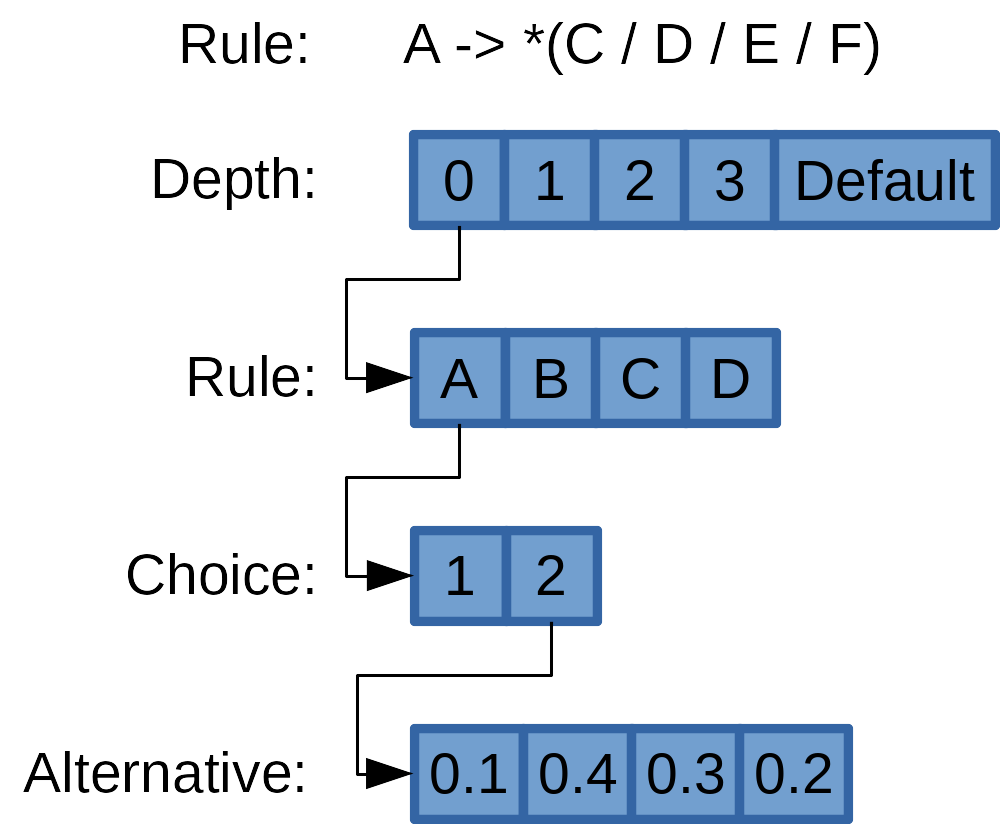
\includegraphics[width=0.6\textwidth]{figures/distribution}
    \caption[Example grammar distribution]{Example grammar distribution applied to the second choice of rule $A$ at depth 0.}
    \label{fig:distribution}
\end{figure}

By using a specialized distribution, rather than a uniform distribution, the generator may be targeted at specialized L-systems, or just have a higher average fitness score for the generated plants.
For example, the distribution may focus more on producing the \textit{F} character which is used for drawing the branch segments.
Or it may be focused on the \textit{stack} rule that produces branch bases.
This may in turn increase the rate of produced plants that have long or many branches.

In addition to the distribution weights shown in Figure~\ref{fig:distribution}, there is a default distribution that will be used if there does not exist a mapping for a rule and choice at a specific depth.
This can be used to prevent infinite recursion with the \textit{stack} rule.
For example, the distribution for the grammar in Listing~\ref{lst:grammar} may specify the weights $[0.5, 0.5]$ for the second choice (\textit{symbol / stack}) in the \textit{string} rule at depth 0, 1 and 2, such that there is an equal change to produce a string and a stack (branch base).
To prevent any deeper branch bases, the weights $[1.0, 0.0]$ may be specified for the default distribution, causing it to not produce a stack at depth 3 or deeper.

To find specialized distributions to more efficiently generate good plants or generate different types of plants, the weights in the distribution need to be optimized.
As the distribution maps from depth, to rule, to choice, to alternative (weight), it is a four-dimensional parameter space to be optimized.
DGEL uses Simulated Annealing (SA) to perform the optimization, but other multi-dimensional parameter optimizers could just as well be used.

Specifically, DGEL implements the basic SA approach~\cite{2000Ozdamar}, as described by Onbaşoğlu and Özdamar~\cite{2001Onbasoglu}.
The only difference is that the initial solution is not initialized randomly, but initialized from a pre-optimized solution, such that it has a better starting point.
In the DGEL SA, the \textit{solution} is the distribution itself, filled with weights for each of the alternatives in each of the choices in each of the rules in a limited set of depths.

A neighbor solution is generated in the same manner as Onbaşoğlu and Özdamar describes~\cite{2001Onbasoglu}: selecting one single random weight and either increasing or decreasing the weight randomly, bounded to the range $[0.0, 1.0]$ in the case of DGEL.
A key difference is that since these are \textit{weights}, the remaining weights in the same set of weights have to be modified such that the sum of all of the weights equal 1.
If the sum of the remaining weights is greater than 0, they can be scaled by a normalization factor, calculated by $\frac{(1 - w)}{(1 - w_0)}$, where $w$ is the new value of the modified weight, and $w_0$ is the old value of the modified weight.
If the sum of the remaining weights is exactly 0, scaling the weights will not work, as they would remain 0.
The alternative solution is to divide the ``remaining weight'' over the remaining weights.
This is done by setting the remaining weights to $\frac{(1 - w)}{(n - 1)}$, where $w$ is the new value of the modified weight, and $n$ is the number of weights.

Accepting a neighbor solution also follows the same approach as Onbaşoğlu and Özdamar describes~\cite{2001Onbasoglu}.
To do this, an $f(x)$, where $x$ is a grammar distribution, has to be defined.
The performance of a grammar distribution can not directly be measured, but it can be estimated by measuring the average performance of the L-systems it generates.
As the performance of the L-systems generated may vary by a big degree, the average performance, $mean$, is only accepted after a specified amount of L-systems, $n$, have been generated, and the standard error of the performance, $se$, is below a threshold value, $t$ (Algorithm~\ref{alg:eval-dist}).

\begin{algorithm}
\caption{Distribution evaluation}
\label{alg:eval-dist}
\begin{algorithmic}
\Function{evaluate\_dist}{$dist$, $n$, $t$}
    \State $samples\gets \Call{empty\_list}{}$
    \State $mean\gets UNDEFINED$
    \State $se\gets INFINITE$
    \While {$se\geq t$}
        \State $new\_samples\gets \Call{generate}{$n$, $dist$}$
        \State $samples\gets \Call{concat}{$samples$, $new\_samples$}$
        \State $mean\gets \Call{mean}{$samples$}$
        \State $se\gets \Call{standard\_error}{$samples$}$
    \EndWhile
    \State \Return $mean$
\EndFunction
\end{algorithmic}
\end{algorithm}

\section{Using Grammar Evolution to Search the Space}
The main component of DGEL is the Grammar Evolution (GE) of the L-systems, which is used to search the parameter space for the best L-system.
The GE process takes a grammar description and a grammar distribution as the input, and produces a single L-system chromosome as the output.

It follows the process as described by Ryan et al.~\cite{1998Ryan}, but with some modifications to the representation as described in Section~\ref{sec:grammar}.
Ryan et al.\ do not describe the selection strategy they used, while Beaumont and Stepney use a simple selection strategy where a percentage of the best individuals are selected as parents~\cite{2009Beaumont}.
Since GE is a specialization of GA, GE can use the same selection strategies as GA.
Thus, tournament selection was selected for DGEL, based on Blickle and Thiele's structured comparison of selection strategies~\cite{1995Blickle}, and Razali and Geraghty's comparison of selection strategies applied to the traveling salesman problem~\cite{2011Razali}.
Both tournament and ranking selection are recommended as good options, but tournament selection performs faster~\cite{1995Blickle}.
Thus because it is assumed that DGEL may be used in real-time applications, tournament selection is preferred.

To make the choice of tournament selection based on Blickle and Thiele's comparison to be valid, the GE algorithm is implemented as GA is described in the same paper.

\section{Using a Fitness Function to Evaluate Plants}
A crucial component of both the SA and GE process is the fitness function.
The fitness function is used by SA to evaluate the grammar distributions, and by GE to evaluate individual L-systems.
Its function is to evaluate how ``good'' the L-system plants are, or more specifically how ``aesthetically pleasing'' they are.
The literature on evolutionary L-systems generally aim the fitness function at evaluating how realistic the plants are by using metrics such as its light gathering ability, positive phototropism and structural stability.

It is assumed that a baseline for aesthetically pleasing plants is that they look at least somewhat realistic, otherwise they would not look like plants at all.
Thus, the metrics used for the fitness function in DGEL uses metrics from the literature, or metrics inspired from the literature, where the metrics usually are targeted towards realistic plants.
Additionally, the metrics were improved upon by generating a plants and looking for bad features in well-scored plants.
Following Ochoa~\cite{1998Ochoa}, each metric is weighted so that their importance may be tuned.
Table~\ref{tab:fitness} lists all of the metrics and their weight.

\begin{table}
    \centering
    \begin{tabularx}{\textwidth}{| l | X | l | l |}
    \hline
    \textbf{Metric} & \textbf{Description} & \textbf{Equation} & \textbf{Weight} \\
    \hline
    Nothing & Punish plants that have no branches (can not be seen) & \ref{eq:nothing} & 1 \\
    \hline
    Closeness & Punish plants with child branch segments very close to each other & \ref{eq:closeness} & 1 \\
    \hline
    Drop & Punish plants based on how much the plant grows downwards & \ref{eq:drop} & 1 \\
    \hline
    Balance & Reward plants that have their center of gravity closer to their root & \ref{eq:balance} & 1 \\
    \hline
    Branching & Reward plants with a balanced number of child branches & \ref{eq:complexity} & 1 \\
    \hline
    Foliage & Reward plants with more leaves & \ref{eq:foliage} & 1.5 \\
    \hline
    Length & Reward longer plants & \ref{eq:length} & 1 \\
    \hline
    Curvature & Reward plants that have somewhat curving branches & \ref{eq:curvature} & 0.4 \\
    \hline
    \end{tabularx}
    \caption{Fitness metrics}
    \label{tab:fitness}
\end{table}

\textit{Nothing} is the simplest and most basic metric.
It punishes plants that have no branch segments.
This may happen if for example the L-system contains no drawing commands (the character \textit{F}).
Equation~\ref{eq:nothing} demonstrates this by giving it a score of -1 if it does not have any branch segments.
In this case no other metrics will make any difference.
The $branches$ function returns the number of branch segments.

\begin{equation}
\label{eq:nothing}
    nothing(x) =
    \begin{cases}
        0,& \text{if } branches(x) > 0  \\
        -1,& \text{otherwise}
    \end{cases}
\end{equation}

\textit{Closeness} is another punishing metric that punishes plants that have branch bases with child segments too close to each other.
This metric helps avoid plants that have segments clipping into each other.
This clipping may look bad, and if they are completely inside each other the complexity of the 3D model increases, which decreases the rendering performance without improving visuals.
The dot product between the direction of two child segments is used for this metric.
The dot product is larger the closer the direction vectors are, becoming 1 when they are parallel.
If the largest dot product between segment directions in a branch base is below a threshold, $t$, there is no punishment.
Otherwise, the plant is punished by a factor depending on how much above the threshold the dot product is.
This factor is interpolated between 0 and 1 linearly from the threshold to 1.
Equation~\ref{eq:closeness} shows how the closeness is calculated.
The $closest$ function finds the closest dot product between child segments in a branch base.
The threshold was experimentally set to 0.9 to punish plants that have segments that look like they clip into each other.

\begin{equation}
\label{eq:closeness}
    closeness(x) =
    \begin{cases}
        0,& \text{if } closest(x) < t \\
        -\frac{c - t}{(1 - t)},& \text{otherwise}
    \end{cases} \\
\end{equation}

\textit{Drop} is a third punishing metric that punishes plants that grow downwards.
It finds the lowest point on the plant, and punishes the plant if it is below 0.
Equation~\ref{eq:drop} demonstrates this.
The $lowestpoint$ function returns the smallest value of the y-component of all points on the plant.
This value is then clamped in the range -1 and 1 and interpolated using a sine function to quickly increase the punishment.
Thus plants where the lowest point is 0 or above will not be punished, while on plants where it is -1 or below will be punished by -1.

\begin{equation}
\label{eq:drop}
drop(x) = sin(clamp(lowestpoint(x), -1, 0) * \frac{\pi}{2})
\end{equation}

\textit{Balance} is a measure of how well balanced the weight of the plant is.
It is inspired by the Bilateral Symmetry measure by Ochoa where 2D plants that reach equally long both left and right are rewarded the most~\cite{1998Ochoa}.
A different approach has to be taken in 3D where there are not only two horizontal directions, but rather an infinite number.
The approach taken is to estimate where the center of gravity of the plant is, calculate the horizontal distance, $centerdistance$, to it, and compare it to how far the plant reaches, $centerspread$, in the horizontal direction of the center of gravity.
This is done by Equation~\ref{eq:balance}.
In the worst case, if both $centerdistance$ and $centerspread$ are the same, the plant will be punished by -1.
In the best case, if the $centerdistance$ is 0, i.e.\ the gravitational center is in the center of the plant, the plant will be rewarded by 1.
Since $centerdistance$ generally will increase with increasing $centerspread$, the plant will be more punished the more it spreads out in one direction.
Though by having most of its branch segments close to the root, it may mitigate the punishment.
Thus the fraction $\frac{centerdistance}{centerspread}$ is used.

\begin{equation}
\label{eq:balance}
balance(x) = (0.5 - \frac{centerdistance(x)}{centerspread(x)}) * 2
\end{equation}

\textit{Branching} measures how complex the branching of the plant is.
It is inspired by the Structural Stability~\cite{1998Ochoa}, Plant Structural Stability~\cite{2009Corchado} and Proportion of Branch Bases~\cite{1998Ochoa} measures.
These measures assume that the plant becomes too unstable to survive if it has too many child segments growing from a branch base.
Corchado et al.\ additionally assume that plants with too few branches will have worse light gathering ability.
Thus there will be a sweet spot in the branching proportion which is rewarded the most.
If the proportion is too low or too high, the plant will be punished.
This is shown in Equation~\ref{eq:complexity} where if the branching proportion is below 1.2 (1.2 child segments from a branch base on average), or above 5, it will be punished in range $[-1, 0]$.
While between 1.2 and 5, it will be rewarded in range $[0, 1]$.
The sweet spot is 2, where it will be rewarded by 1.
$icos$ interpolates the value from the first parameter, $a$, to the second parameter, $b$, using a cosine function.
The third parameter, $t$, is in range $[0, 1]$ and controls where between $a$ and $b$ the interpolation is.
This creates a smooth curve between the limits.

\begin{equation}
\label{eq:complexity}
\begin{aligned}
    branching(x) =
    \begin{cases}
        -1, & b < 1 \\
        icos(-1, 0, \frac{b - 1.0}{0.2}), & b < 1.2 \\
        icos(0, 1, \frac{b - 1.2}{0.8}), & b < 2 \\
        1, & b < 3 \\
        icos(1, -1, \frac{b - 3}{5.8}), & b < 7 \\
        -1, & \text{otherwise}
    \end{cases}, \\
    \text{where } b = \frac{branches(x)}{branchings(x)}
\end{aligned}
\end{equation}

\textit{Foliage} measures how many leaves a plant has.
It is the main metric for measuring the light gathering ability of the plant, and is inspired by Ochoa~\cite{1998Ochoa}, Ebner~\cite{2003Ebner}, and Corchado et al.'s~\cite{2009Corchado} light gathering ability metrics.
The main point is that more leaves exposed to sunlight means that the plant has a better ability to survive.
For simplicity, the metric used in DGEL is based on Corchado et al.'s metric which simply rewards plants with more leaves~\cite{2009Corchado}.
It also counts leaves that are shadowed by other leaves, even though in reality these would gather only minimal amounts of light.
This selection of method was due to time constraints, and a more complex method like Ebner's would be better.
The metric used starts with a reward of 0 for 0 leaves and is asymptotic towards 1 when the leaf count, found by $leaves$, increases towards $\infty$.
Equation~\ref{eq:foliage} demonstrates this.
The $s$ constant controls how fast it should increase towards 1.

\begin{equation}
\label{eq:foliage}
    foliage(x) = \frac{leaves(x) * s}{1 + leaves(x) * s}, \text{where } s = 0.1
\end{equation}

\textit{Length} rewards plants that are longer.
It is inspired by Ochoa and Corchado et al.'s Positive Phototropism metrics where the assumption is that plants grow towards the sunlight and thus taller plants are better at surviving.
While Positive Phototropism only cares about the height of the plant, Length cares about how long the plant is, not considering if it grows upwards or not.
This change is made on the assumption that plants can gather more light both by growing upwards (cover more vertical area) and sideways (cover more horizontal area).
Additionally it was found during an early experiment that short plants were generally found as displeasing.
Like the Foliage metric, the Length metric is asymptotic towards 1 as the plant length increases towards $\infty$.
This is shown in Equation~\ref{eq:length}.
The length of the plant is found using $longest$, which finds the longest path in the branches of the plant from root to leaf and returns the number of branch segments in it.
As with the Foliage metric, the $s$ constant controls how fast it should increase towards 1.

\begin{equation}
\label{eq:length}
    length(x) = \frac{longest(x) * s}{1 + length(x) * s}, \text{where } s = 0.5
\end{equation}

\textit{Curvature} is a metric that rewards plants with more curved branches.
It was developed from the results of the first experiment where it was found that plants that looked ``static'' or ``straight'' were not as pleasing as plants that looked more ``dynamic'' or ``curvy''.
As Equation~\ref{eq:curvature} demonstrates, the plant is rewarded more if the branch segments are oriented with a small angle different from their parent.
If the angle is too sharp, the plant is rewarded less, as the plant may look like ``doodles'' with such angles.
The $minangles$ function returns a list of the smallest angle from an internode segment to its parent segments.
Thus, if an internode segment only has one child (i.e.\ it does not branch), the smallest angle will be the angle between it and that one child.
Otherwise, if an internode segment has multiple children (i.e.\ it is a branch base), all of the angles between it and the children are calculated and the smallest will be used.
This is based on the assumption that the child segment with the smallest angle is the straight segment following a branch base.
% This assumption only holds for apex trees? What if it branches into two equally angled branches?
$avg$ calculates the average of all of the angles returned by $minangles$.
Like in Equation~\ref{eq:complexity}, $icos$ is used to create a smooth interpolation between the limits $min$, $opt$ and $max$.
A sweet spot of $opt = 0.24711092$, which is rewarded by 1, was found to provide a good curvature in the plant.
A limit of $max = \frac{\pi}{4}$ (45°) was intuitively chosen as a point where the curvature is no longer rewarding.

\begin{equation}
\label{eq:curvature}
\begin{aligned}
    curvature(x) =
    \begin{cases}
        icos(0, 1, \frac{a - min}{opt - min}), & a >= min \text{ and } a < opt \\
        icos(1, 0, \frac{a - opt}{max - opt}), & a >= opt \text{ and } a < max \\
        min, & \text{otherwise}
    \end{cases}, \\
    \text{where } a = avg(minangles(x)), \\
    min = 0, \\
    opt = 0.24711092, \\
    max = \frac{\pi}{4} \\
\end{aligned}
\end{equation}

% REMEMBER TO MENTION THAT TERMS USED ARE BASED ON AXIAL TREES IN L-SYSTEM BOOK.
